\documentclass[tikz,border=4pt]{standalone}
\usepackage{amsmath}
\usetikzlibrary{arrows.meta,positioning,calc}
\begin{document}
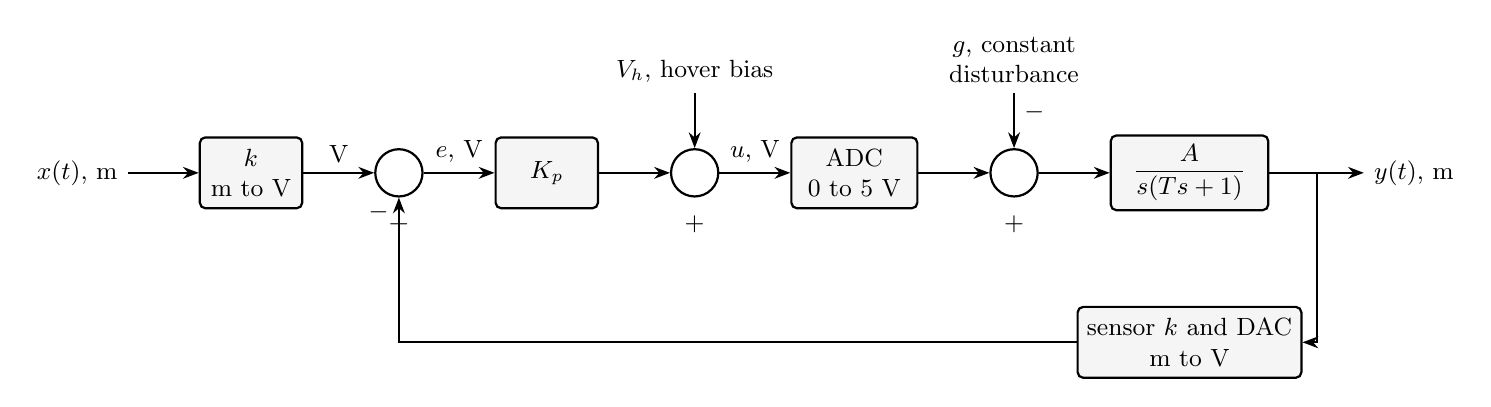
\begin{tikzpicture}[
  >={Stealth[length=2mm]},thick,font=\small,
  blk/.style={draw,rounded corners=2pt,minimum height=9mm,minimum width=13mm,align=center,fill=gray!8},
  sum/.style={draw,circle,inner sep=1pt,minimum size=6mm},
  node distance=9mm and 9mm]

  \node (x) {$x(t)$, m};
  \node[blk,right=of x] (ks) {$k$\\m to V};
  \node[sum,right=of ks] (e) {};
  \node[blk,right=of e] (kp) {$K_p$};
  \node[sum,right=of kp] (shift) {};
  \node[blk,right=of shift,minimum width=16mm] (adc) {ADC\\$0$ to $5$ V};
  \node[sum,right=of adc] (dsum) {};
  \node[blk,right=of dsum,minimum width=20mm] (plant) {$\dfrac{A}{s(Ts+1)}$};
  \node[right=12mm of plant] (y) {$y(t)$, m};

  \node[above=7mm of shift,align=center] (vh) {$V_h$, hover bias};
  \node[above=7mm of dsum,align=center] (g) {$g$, constant\\disturbance};

  \node[blk,below=12mm of plant,minimum width=20mm] (dac) {sensor $k$ and DAC\\m to V};

  \draw[->] (x) -- (ks);
  \draw[->] (ks) -- node[above] {V} (e);
  \draw[->] (e) -- node[above] {$e$, V} (kp);
  \draw[->] (kp) -- (shift);
  \draw[->] (vh) -- (shift);
  \draw[->] (shift) -- node[above] {$u$, V} (adc);
  \draw[->] (adc) -- (dsum);
  \draw[->] (g) -- node[right,pos=0.35] {$-$} (dsum);
  \draw[->] (dsum) -- (plant);
  \draw[->] (plant) -- (y);

  \coordinate (tap) at ($(plant.east)+(6mm,0)$);
  \draw[->] (tap) |- (dac.east);
  \draw[->] (dac.west) -| node[pos=0.95,left] {$-$} (e);

  \node[below=1mm of e] {$+$};
  \node[below=1mm of shift] {$+$};
  \node[below=1mm of dsum] {$+$};
\end{tikzpicture}
\end{document}
